% Канонический TikZ-рисунок варианта 36. Править только здесь.
\long\def\figStereoV36{%
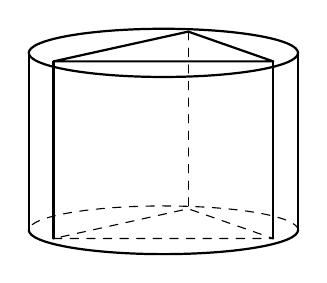
\begin{tikzpicture}[
  scale=0.9,
  line cap=round,
  line join=round
]
  \def\R{1.9}
  \def\H{2.5}
  \def\e{0.34}

  % Вершины верхнего основания призмы
  \coordinate (T1) at (-1.55,2.38);
  \coordinate (T2) at ( 1.55,2.38);
  \coordinate (T3) at ( 0.35,2.80);

  % Вершины нижнего основания призмы
  \coordinate (B1) at (-1.55,-0.12);
  \coordinate (B2) at ( 1.55,-0.12);
  \coordinate (B3) at ( 0.35, 0.30);

  % Верхнее основание цилиндра
  \draw[thick]
    (0,\H) ellipse[x radius=\R,y radius=\e];

  % Образующие цилиндра
  \draw[thick] (-\R,0)--(-\R,\H);
  \draw[thick] ( \R,0)--( \R,\H);

  % Нижнее основание цилиндра
  \draw[thick]
    (-\R,0)
    arc[
      start angle=180,
      end angle=360,
      x radius=\R,
      y radius=\e
    ];

  \draw[dashed]
    (\R,0)
    arc[
      start angle=0,
      end angle=180,
      x radius=\R,
      y radius=\e
    ];

  % Верхнее основание призмы
  \draw[thick]
    (T1)--(T2)--(T3)--cycle;

  % Нижнее основание призмы
  \draw[dashed]
    (B1)--(B2)--(B3)--cycle;

  % Боковые рёбра призмы
  \draw[thick]  (T1)--(B1);
  \draw[thick]  (T2)--(B2);
  \draw[dashed] (T3)--(B3);
\end{tikzpicture}
}
